\section{Apache Mesos:}
\label{sec:mesos}
Mesos was started in 2009 to try and increase the performance and utilization of clusters. The project's key idea was to have a framework for the distributed system so that  the nodes in a cluster can be used as a shared pool instead of statically partitioning each of those individual nodes (filip). 

Usually in a static sharing or static partitioning, one server runs on one node availing all its resources. Most of the times, the resources on such nodes are wasted as the server doesn't utilize all the resources of the node. Using the elastic sharing, Mesos layer of abstraction talks to all the available nodes in the cluster aggregating the resources, making a cluster of nodes look like as one single machine.

\begin{figure*}
\centering
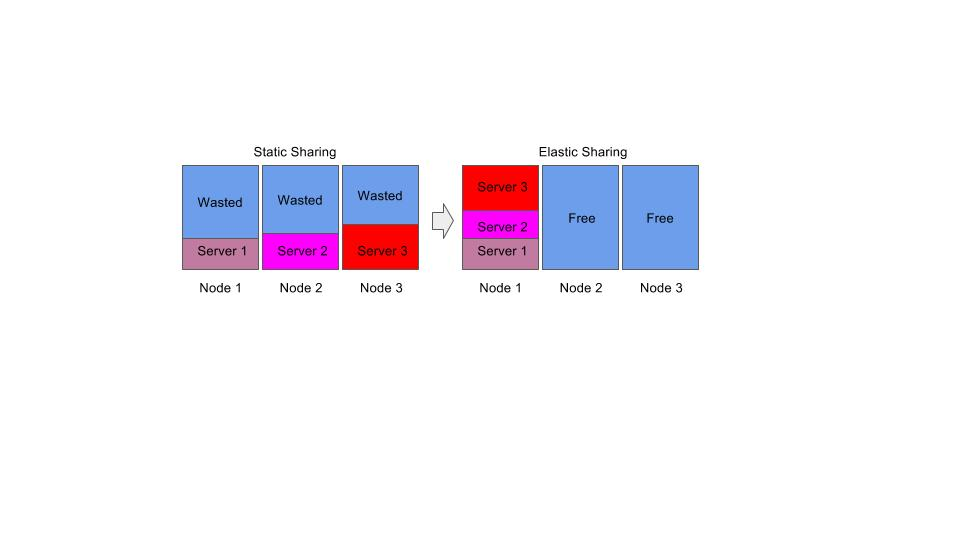
\includegraphics[scale=0.5]{./fig/elastic_sharing}
\caption{Elastic Sharing in Mesos}
\label{fig:elastic_sharing}
\end{figure*}

As shown in figure 2, Mesos architecture consists of master nodes and agent nodes, framework and Zookeeper. In Mesos cluster, Master nodes run the master process that manages the slave processes running on agent nodes. Slave processes run the tasks, for e.g. a database query or bash command, which are scheduled to be executed on the agent nodes. 

Framework is a Mesos application which has has two component: scheduler and executor. Using their scheduler, framework schedules the task to run on the agent nodes. The tasks are executed by executor process that is launched on each agent nodes. Before scheduling a task, framework needs to be registered with the master node. The services running on the top of the Mesos framework don't care about the cluster resources. The services/frameworks running on top of the Mesos requests to the Mesos layer for the resources required at that particular time.

Master node offers the available resources on the agent nodes to the registered framework. These offered resources are the list of free resources on the agent nodes. Master node gets the information about the available resources from the agent nodes and it decides how many resources to be offered to frameworks. Master node makes this offer by having the nearest approximation of the available resources which matches the framework's request. Master node only offers the available resources to the registered frameworks.
 
After receiving the offer, the framework, e.g. Marathon or Hadoop, chooses to accept or reject the offer. It can reject the current offer and wait for the offer which satisfies their request. If the offer is accepted then the framework deploys the task on the agent node. Once the task is completed, the resources are freed up by the master node. 

Zookeeper is a tool which is used provide the high availability of the master nodes in Mesos. It replicates the master nodes and coordinate with them. One of these masters is selected as the leader.

\begin{figure*}
\centering
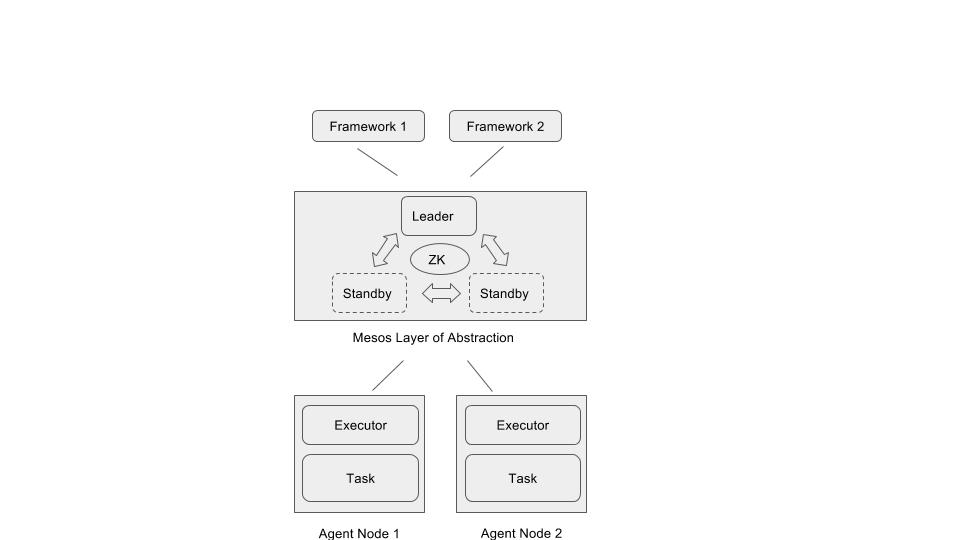
\includegraphics[scale=0.5]{./fig/mesos}
\caption{Apache's Mesos Architecture}
\label{fig:mesosArch}
\end{figure*}

Following are the features of Mesos:

\begin{enumerate}
\item High Availability: Mesos provides high availability of master node by having multiple replicas of the master node. It uses Zookeeper tool to replicate the master node and coordinate between these replicas. However, Mesos doesn't provide fault tolerance for the application failure. It only detects the failure, but doesn't handle it.

\item Linear Scalability: Mesos framework is easily scalable to tens of thousand nodes.

\item Resource Isolation: Using Linux containers, Mesos provides performance isolation between tasks of different frameworks on the same agent node.

\item Fault Tolerance: In case of node failure, Mesos notifies the framework about the node failure and its executor. Depending ontheir policies, the framework acts on those notifications.

In Mesos, frameworks are allowed to have multiple schedulers to be registered with master node. In case one of the scheduler fails, the Mesos master will notify the another scheduler to take over. Sharing the state between the schedulers is upto the frameworks.

\item Cross Platform support: Mesos can run on different platform like Linux, Windows and OSX.

\item Two level scheduling: Using the resource offer technique, Mesos separates the resource management and process scheduling.  Mesos master decides about the resources to be offered to the frameworks, while frameworks decides how to manage their distributed processes. Frameworks uses short tasks and elastic resource utilization to improve the response time of the tasks.

\item HTTP APIS: Mesos provides HTTP APIs to monitor and operate cluster and to develop new distributed applications.
WEB UI

\end{enumerate}



















